\documentclass{beamer}

\mode<presentation>{\usetheme{poster}}

% Load packages here
\usepackage{amsmath,amssymb,array}
\usepackage{graphicx,tcolorbox}
\tcbuselibrary{listings,breakable,most,hooks,skins}
\graphicspath{{./graphics/}}
\usepackage[orientation=landscape,size=custom,width=48,height=36,scale=.6,debug]{beamerposter}
\usepackage{mathptmx}
\usepackage{verbatim}
\renewcommand\sfdefault{ptm}
\def\Z{\mathbb Z}
\def\N{\mathbb N}
\def\Q{\mathbb Q}
\def\R{\mathbb R}
\def\C{\mathbb C}
\def\F{\mathbb F}
\def\P{\mathbb P}
\def\E{\mathbb E}
\def\G{\mathbb G}
% Header and footer 
\newcommand{\footleft}{http://mcl.math.uic.edu/}
\newcommand{\footright}{}
\title{Vietoris-Rips complexes, ravfndom points on varieties, and persistent homology}
\author{Daniel Etrata \quad Mason Boeman}
\institute{Mentors: Benjamin Antieau and J\={a}nis Lazovskis}

% Main document
\begin{document}
\begin{frame}{}
\begin{columns}[t]

%-- Column 1 ---------------------------------------------------
\begin{column}{0.32\linewidth}

%-- Block 1-1
\begin{block}{Summary}

The project takes a variety of n-dimensions intersected by random lines to generate points. From this point cloud, an undirected neighborhood graph is constructed, where then the edges are assigned a weight. Then, the neighborhood graph undergoes the Vietoris-Rips expansion by constructing cofaces for which the vertex is maximal.
\end{block}



%-- Block 1-2
\begin{block}{Motivation}
The goal of this project is to use persistent homology to study the topology of random complex algebraic varieties, geometric figures described as the solution sets of system of polynomial equations. 

\end{block}

%-- Block 1-3
\begin{block}{Using PHCpack to find points}
PHCpack is a polynomial system solver using homotopy continuation methods. Let $f(x) = 0$ be the target system. PHC constructs $g(x)=0$ start system. Then let $\gamma$ be the accessibility constant, $\gamma \in \C$ and $t$ be the continuation parameter, $t \in [0,1]$. The homotopy $h$ is defined as
\begin{equation*}
h(x,t) = \gamma \cdot (1-t)\cdot g(x) + t \cdot f(x) = 0
\end{equation*}
\begin{equation*}
h(x, 0) =g(x)
\end{equation*}
\begin{equation*}
h(x, 1) = f(x)
\end{equation*}
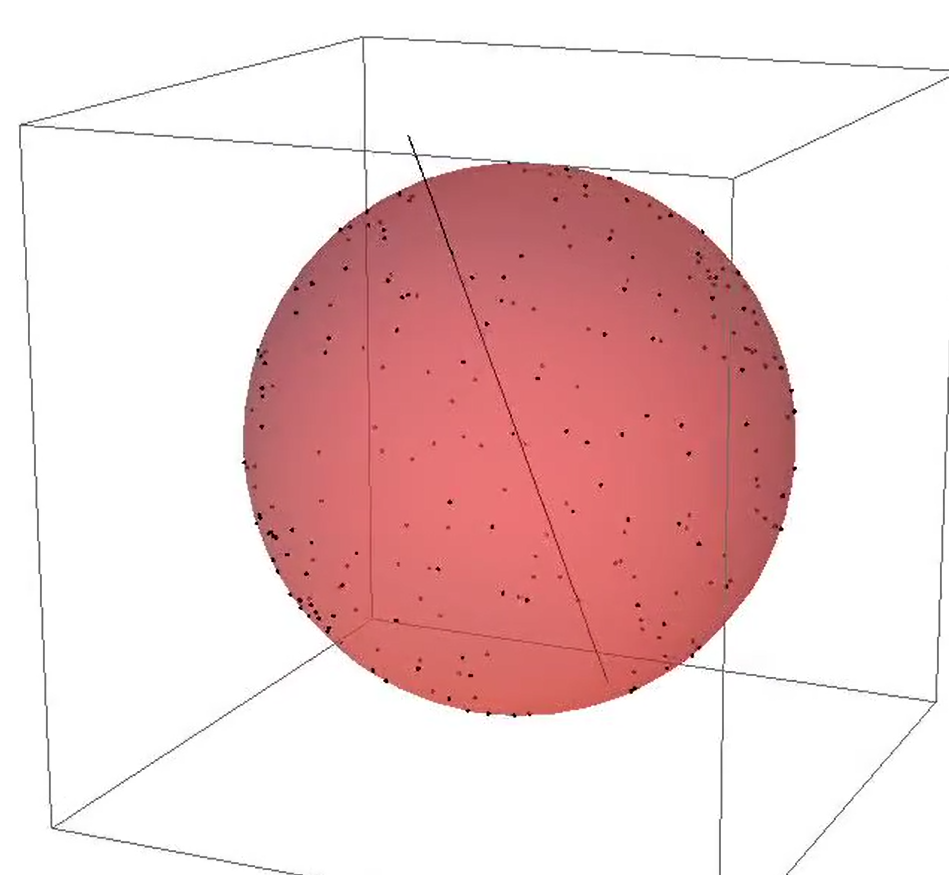
\includegraphics[width=.5\columnwidth]{sphere}
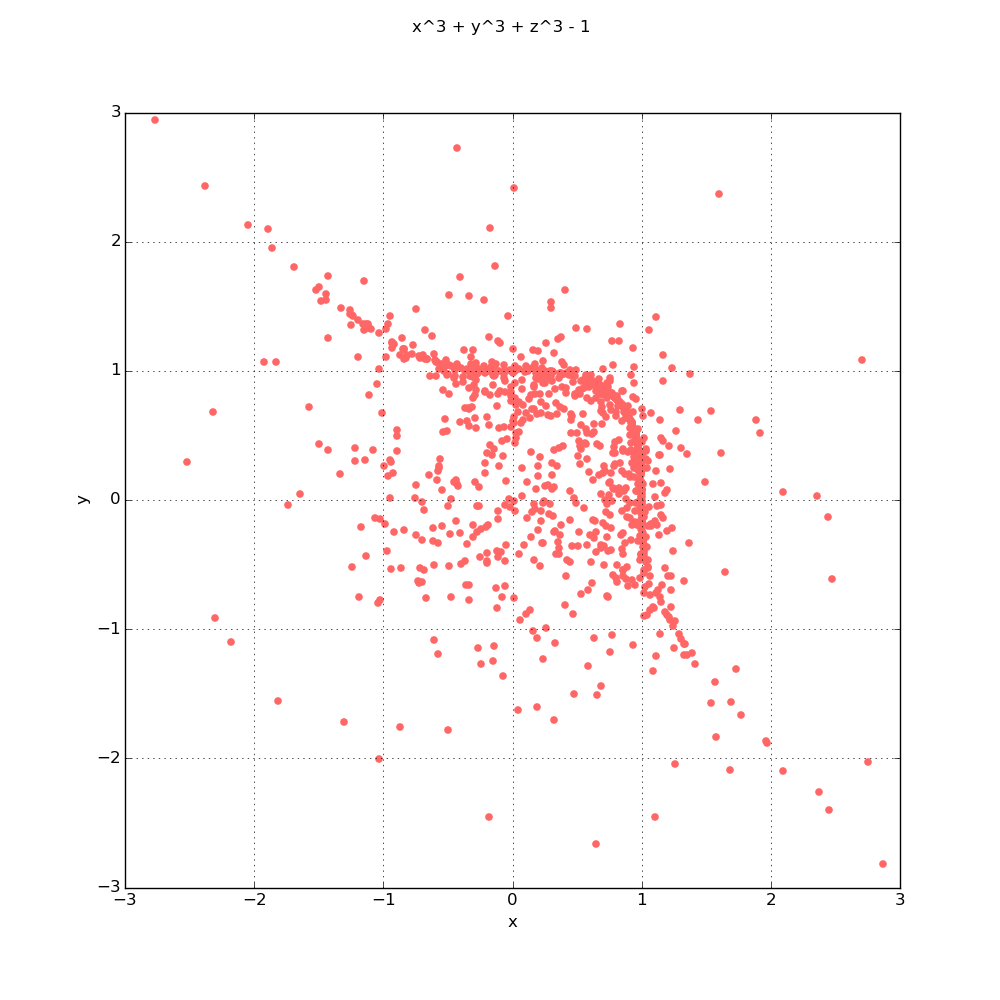
\includegraphics[width=.5\columnwidth]{plot2d_5}


\end{block}


\end{column}%1

%-- Column 2 ---------------------------------------------------
\begin{column}{0.32\linewidth}

%-- Block 2-1
\begin{block}{Neighborhood graphs}
\centering
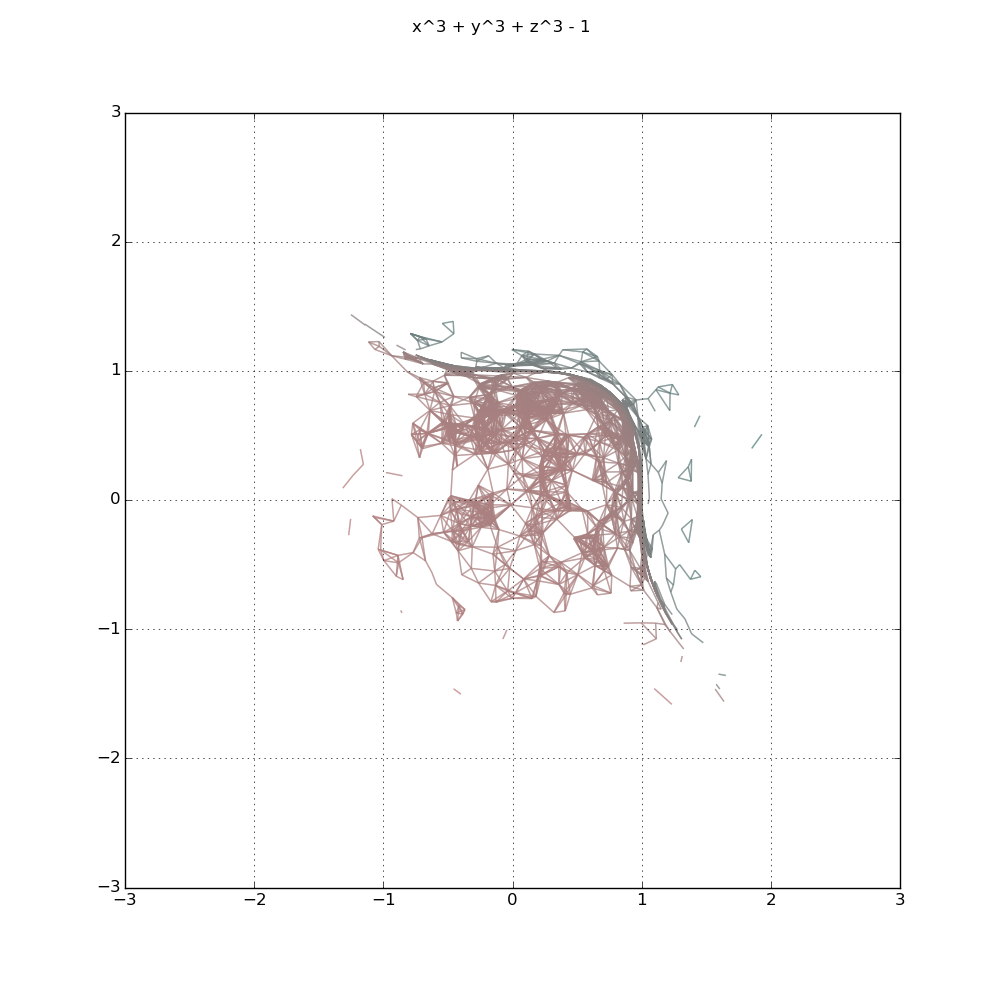
\includegraphics[width=1\columnwidth]{plot2d_ng_7}

\end{block}

%-- Block 2-2
\begin{block}{Vietoris-Rips complex}

\end{block}

%-- Block 2-3
\begin{block}{Pictures}
\begin{figure}[htb]

\end{figure}
\end{block}

\end{column}%2

%-- Column 3 ---------------------------------------------------
\begin{column}{0.32\linewidth}

%-- Block 3-1
\begin{block}{Persistent homology}

\end{block}

%-- Block 3-2
\begin{block}{Experiments}

\end{block}

%-- Block 3-3
\begin{block}{Conclusion}

\end{block}

\end{column}%3

\end{columns}
\end{frame}
\end{document}
